\section{Relationship to the Koenigs function}\label{a:sec:koenigs}
\label{a:sec:koenigs-link}

The preceding recurrence already has the form of a logistic iteration.  This
section makes its connection with classical Koenigs linearisation precise and then
uses that connection to formulate the closed-form obstruction for $r\in(0,1)$.

\subsection{From the survival recurrence to the logistic map}

Recall that
\[
S_{n+1}=2p\,S_n-p\,S_n^2,\qquad S_0=1,
\]
and $A(p)=\lim_{n\to\infty}S_n/(2p)^n$. Setting $S_n=2w_n$ and $r=2p$ yields the logistic iteration
\begin{equation}
\label{a:eq:logistic-koenigs}
w_{n+1}=f_r(w_n),\qquad f_r(w)=r w(1-w),\qquad w_0=\tfrac12,
\end{equation}
with $r\in[0,1)$ throughout the subcritical regime.  Consequently,
\begin{equation}
\label{a:eq:A-from-w}
A(p)=2\lim_{n\to\infty}\frac{w_n}{r^n}.
\end{equation}

\subsection{Koenigs linearisation}

\begin{definition}[Koenigs function for the logistic map]
\label{a:def:koenigs}
Let $f_r(z)=r z(1-z)$ have multiplier $r$ at the fixed point $0$, with
$0<|r|<1$.  There exists a unique holomorphic map $\psi_r$, defined in a
neighbourhood of $0$, such that
\begin{equation}
\label{a:eq:schroder}
\psi_r\bigl(f_r(z)\bigr)=r\,\psi_r(z),\qquad \psi_r(0)=0,\qquad \psi_r'(0)=1.
\end{equation}
Equivalently,
\begin{equation}
\label{a:eq:koenigs-limit}
\psi_r(z)=\lim_{n\to\infty} r^{-n} f_r^{\circ n}(z)
\end{equation}
uniformly near the origin \cite{Koenigs1884}.  The normalisation
$\psi_r'(0)=1$ is equivalent to $\psi_r(z)/z\to1$ as $z\to0$.
\end{definition}

\begin{figure}[H]
\centering
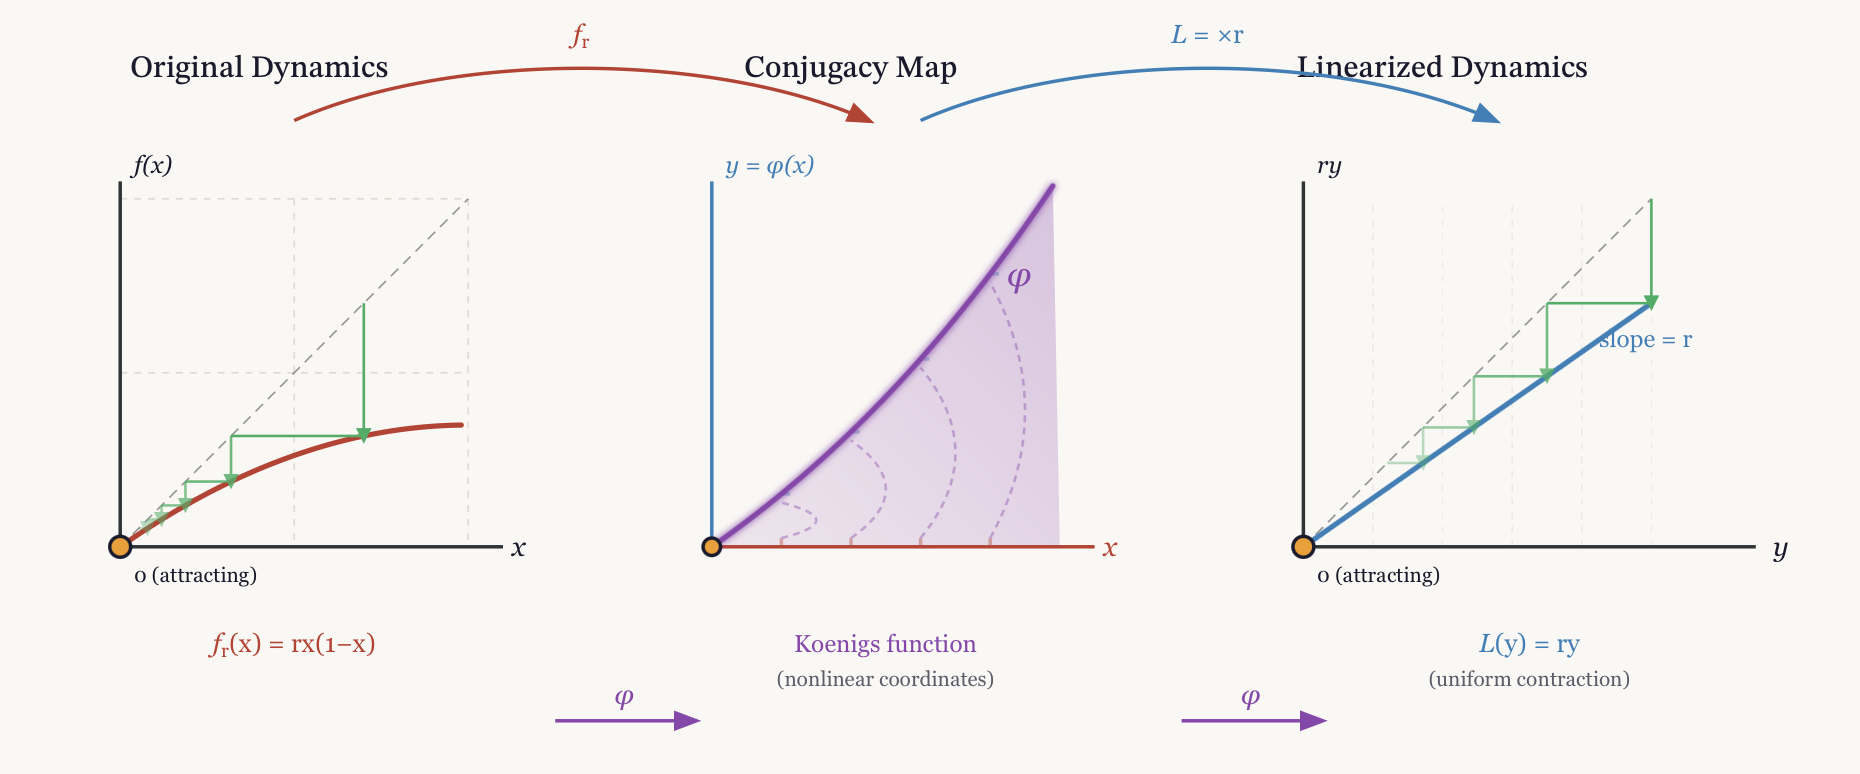
\includegraphics[width=0.78\textwidth]{figures/figure2_koenigs_linearization.png}
\caption{Schematic of Koenigs linearisation: $f_r$ is conjugate, via $\psi_r$, to multiplication by $r$ near the origin.}
\label{a:fig:koenigs-schematic}
\end{figure}

\subsection{The identity \texorpdfstring{$A(p)=2\lim r^{-n}f_r^{\circ n}(\tfrac12)$}{A(p) as a Koenigs value}}

The local Koenigs function is initially defined only near $0$.  For $r\in(0,1)$,
however, the origin attracts the real interval $(0,1)$, and in particular the orbit
from $w_0=\tfrac12$ satisfies $w_n\to0$.  On this basin, the limit
\begin{equation}
\label{a:eq:basin-koenigs}
\Psi_r(w_0)
:=
\lim_{n\to\infty} r^{-n} f_r^{\circ n}(w_0)
\end{equation}
exists and agrees with the local conjugacy near $0$.  Indeed,
$\psi_r'(0)=1$ gives $\psi_r(w)/w\to1$ as $w\to0$, so
$\psi_r(w_n)/r^n\sim w_n/r^n$.  Once the orbit enters the local domain,
\[
\psi_r(w_0)=\frac{\psi_r(w_n)}{r^n};
\]
and passage to the limit yields $\Psi_r(w_0)=\lim w_n/r^n$.  Taking
$w_0=\tfrac12$ and using \eqref{a:eq:A-from-w} gives
\begin{equation}
\label{a:eq:A-koenigs}
A(p)
=
2\Psi_r\bigl(\tfrac12\bigr)
=
2\lim_{n\to\infty} r^{-n} f_r^{\circ n}\bigl(\tfrac12\bigr),
\qquad r=2p\in[0,1).
\end{equation}
The shorthand $A(p)=2\psi_r(\tfrac12)$ will refer to this basin value of the
Koenigs conjugacy, rather than to a direct evaluation of its local power series
beyond the guaranteed disc of convergence.

Questions about an elementary closed form for $A(p)$ are therefore tied to the
nature of the conjugacy at multiplier $r=2p$.
